\chapter{焦点面検出器アライメントの較正}
\label{chapter4}

GroundBIRD実験での偏光測定のためには、検出器間での信号の差分を取ることが重要であり、それに伴って望遠鏡のスキャンに対して最適な検出器のアライメントが求められる。この章では従来の検出器アライメントの最適化に向けた改善を行い、観測データからその効果を確認した。

\section{検出器アライメントの問題点}

\subsection{スキャン軸に対する傾きと差分解析}
まず、GroundBIRDでの解析手法の1つである差分解析と検出器アライメントの関係について述べる。\ref{mkid_design}で示したように、焦点面検出器は異なる偏光方向に感度を持った検出器が交互に配置されている。これらの検出器が検出する信号は空のある点からの放射が望遠鏡内の光学系を経て焦点面へと届いたものである。つまり、焦点面での検出器の配置を空へと射影した時にどう配置されているかが重要になる。各検出器は空のある点を見ており、望遠鏡の方位角回転に伴って同じ仰角の空を回転しながら観測する(図\ref{scan_image})。検出器で観測する信号は大きく(CMB + ノイズ)に分けられる。さらにノイズの中でも寄与が大きい成分に大気揺らぎに由来するノイズがある。

\begin{figure}[htbp]
  \centering
  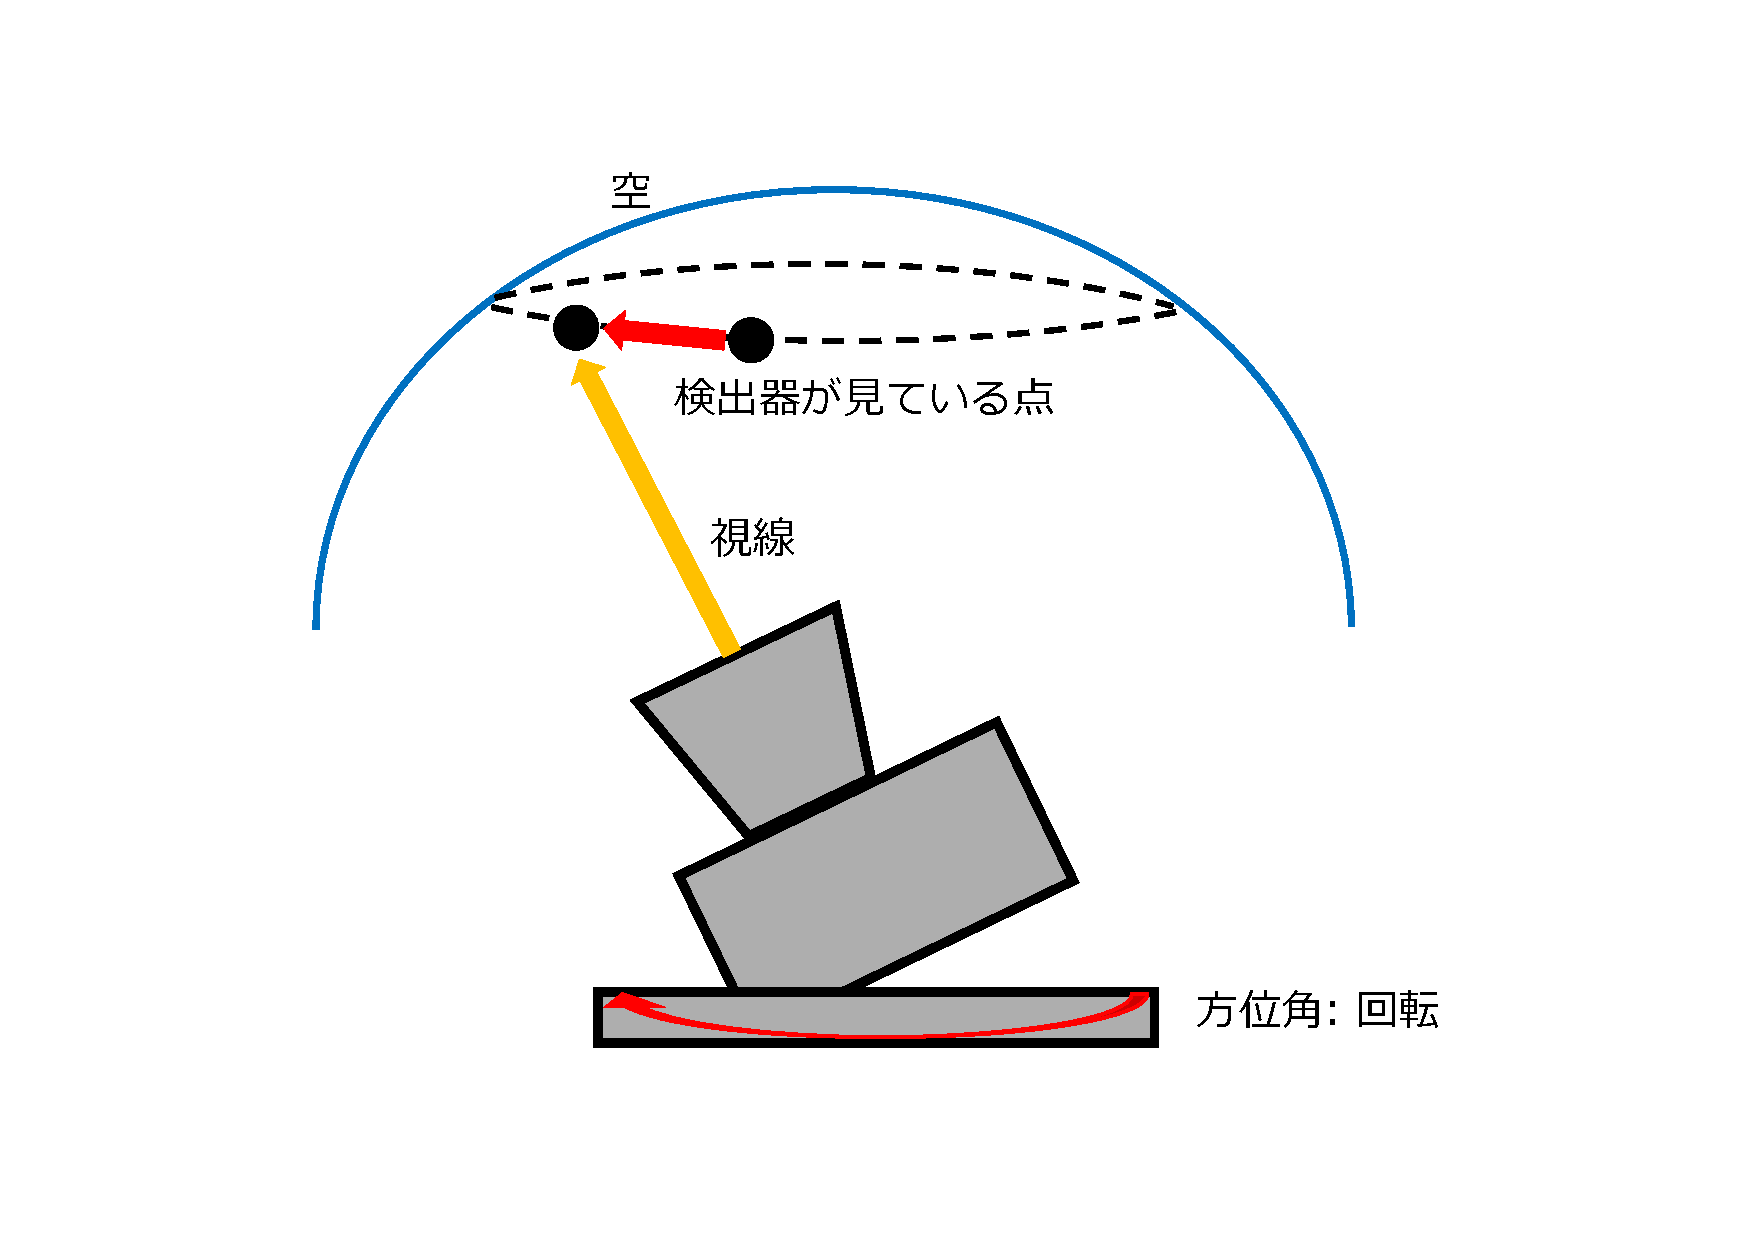
\includegraphics[width=0.6\columnwidth]{5_alignment/figs/scan_image.pdf}
  \caption{検出器が空の領域をスキャンする概要図。ある仰角を高速回転しながらスキャンする。}
  \label{scan_image}
\end{figure}
\subsection{要求されるアライメント性能}

\subsection{視線軸方向まわりの回転による較正}

\section{月を用いた回転角の算出}

\subsection{月を用いた理由}

\subsection{必要な回転角}

\subsection{回転する上でのジグの必要性}

\section{ジグの設計と現地インストール}

\subsection{固定用ジグの作成}

\subsection{望遠鏡への実装}

\section{天体を用いた較正結果の確認}

\subsection{月データによる確認}

\subsection{木星データによる確認}

\section{検出器間差分で見る大気揺らぎの抑制}

\subsection{timing offsetの算出}

\subsection{差分解析による確認}
